% =====================================================================
%  Laboratorio 5 - Seguridad: Patrón de Segmentación de Red
%  Equipo 1-F - Arquitectura de Software 2026-II
%
%  Para Overleaf: subir este archivo junto con vista-arquitectonica.png
%  (mismo nivel). Compilador: pdfLaTeX. Exportar como l5_1f.pdf
% =====================================================================
\documentclass[11pt,letterpaper]{article}

% ---------- Codificación e idioma ----------
\usepackage[T1]{fontenc}
\usepackage[utf8]{inputenc}
\usepackage[spanish,es-noshorthands,es-tabla]{babel}
\DeclareUnicodeCharacter{2192}{\ensuremath{\rightarrow}}
\DeclareUnicodeCharacter{2194}{\ensuremath{\leftrightarrow}}

% ---------- Fuentes ----------
\usepackage{newtxtext}               % texto tipo Times (como la entrega del prototipo)
\usepackage[scaled=0.92]{helvet}     % títulos en sans (como las guías del curso)
\usepackage[varqu,scaled=0.95]{zi4}  % monoespaciada para código

% ---------- Página ----------
\usepackage[margin=2.5cm,headheight=14pt]{geometry}
\usepackage{fancyhdr}
\usepackage{titlesec}
\usepackage{enumitem}
\usepackage{parskip}

% ---------- Tablas, figuras, color ----------
\usepackage[table]{xcolor}
\usepackage{graphicx}
\usepackage{float}
\usepackage{booktabs}
\usepackage{tabularx}
\usepackage{array}
\usepackage{caption}
\usepackage{listings}
\usepackage[hidelinks]{hyperref}

% ---------- Colores (los mismos de la vista arquitectónica) ----------
\definecolor{verde}{HTML}{1B7F3B}
\definecolor{rojo}{HTML}{C0392B}
\definecolor{azul}{HTML}{2D77C9}
\definecolor{gris}{HTML}{5A6B7B}
\definecolor{headbg}{HTML}{DCE6F2}
\definecolor{codebg}{HTML}{F6F6F6}
\definecolor{coderule}{HTML}{D0D0D0}
\definecolor{codecomment}{HTML}{8A8A8A}
\definecolor{codestring}{HTML}{4E8A00}
\definecolor{codekeyword}{HTML}{8E44AD}

\newcommand{\code}[1]{\texttt{#1}}
\newcommand{\ok}[1]{\textcolor{verde}{\textbf{#1}}}
\newcommand{\bad}[1]{\textcolor{rojo}{\textbf{#1}}}
\newcolumntype{Y}{>{\raggedright\arraybackslash}X}

% ---------- Encabezado y pie ----------
\pagestyle{fancy}
\fancyhf{}
\fancyhead[L]{\small\sffamily [SwArch\_2026ii] -- Laboratorio 5: Seguridad}
\fancyhead[R]{\small\sffamily Equipo 1-F}
\fancyfoot[C]{\small\thepage}
\renewcommand{\headrulewidth}{0.4pt}

% ---------- Títulos (estilo de las guías: sans con línea inferior) ----------
\titleformat{\section}{\sffamily\Large\bfseries}{\thesection.}{0.5em}{}
\titleformat{\subsection}{\sffamily\large\bfseries}{\thesubsection.}{0.5em}{}
\titleformat{\subsubsection}{\sffamily\normalsize\bfseries}{\thesubsubsection.}{0.5em}{}
\titlespacing*{\section}{0pt}{2.2ex}{1.4ex}

\captionsetup{font=small,labelfont=bf}
\setlist{itemsep=2pt,topsep=4pt}

% ---------- Bloques de código (estilo de las guías) ----------
\lstdefinelanguage{yaml}{
  morekeywords={true,false},
  sensitive=true,
  morecomment=[l]{\#},
  morestring=[b]",
}
\lstdefinelanguage{nginx}{
  morekeywords={server,listen,location,return,proxy_pass,default_type},
  morecomment=[l]{\#},
  morestring=[b]",
}
\lstdefinelanguage{docker}{
  morekeywords={FROM,RUN,WORKDIR,COPY,EXPOSE,CMD},
  morecomment=[l]{\#},
  morestring=[b]",
}
\lstdefinelanguage{JavaScript}{
  morekeywords={const,let,async,await,return,if,try,catch,require,new},
  sensitive=true,
  morecomment=[l]{//},
  morestring=[b]",
}
\lstdefinelanguage{shell}{
  morekeywords={docker,curl.exe,cd,powershell},
  alsoletter={.},
  morecomment=[l]{\#},
  morestring=[b]',
}

\lstdefinestyle{lab}{
  basicstyle=\ttfamily\small,
  backgroundcolor=\color{codebg},
  frame=single,
  rulecolor=\color{coderule},
  framesep=6pt,
  xleftmargin=6pt,
  xrightmargin=6pt,
  aboveskip=8pt,
  belowskip=8pt,
  columns=fullflexible,
  keepspaces=true,
  breaklines=true,
  showstringspaces=false,
  upquote=true,
  tabsize=2,
  commentstyle=\color{codecomment}\itshape,
  stringstyle=\color{codestring},
  keywordstyle=\color{codekeyword},
  literate=
    {á}{{\'a}}1 {é}{{\'e}}1 {í}{{\'i}}1 {ó}{{\'o}}1 {ú}{{\'u}}1
    {Á}{{\'A}}1 {É}{{\'E}}1 {Í}{{\'I}}1 {Ó}{{\'O}}1 {Ú}{{\'U}}1
    {ñ}{{\~n}}1 {Ñ}{{\~N}}1 {→}{{$\rightarrow$}}1,
}
\lstset{style=lab}

% =====================================================================
\begin{document}

% ---------------------------- Portada --------------------------------
\begin{titlepage}
  \centering
  \vspace*{2.5cm}
  {\LARGE\bfseries LABORATORIO 5: SEGURIDAD\par}
  \vspace{0.5cm}
  {\Large Patrón de Segmentación de Red\par}
  \vspace{0.2cm}
  {\large Guía técnica de implementación\par}

  \vspace{1.6cm}
  {\bfseries PRESENTADO POR:\par}
  \vspace{0.15cm}
  Emiliano Guerra Gallego\par
  Juan Daniel Sossa Solis\par
  Joan Sebastian Vargas Mosquera\par
  Juan Esteban Peña Burgos\par
  Julián David Albarracín Galindo\par
  Michel Mauricio Castañeda Braga\par

  \vspace{1cm}
  {\bfseries MATERIA:\par}
  Arquitectura de Software\par

  \vspace{1cm}
  {\bfseries PROFESOR:\par}
  Jeisson Andrés Vergara Vargas\par

  \vspace{1cm}
  {\bfseries EQUIPO:\par}
  1-F\par

  \vfill
  {\bfseries UNIVERSIDAD NACIONAL DE COLOMBIA\par
  FACULTAD DE INGENIERÍA\par
  BOGOTÁ, NOVIEMBRE DE 2026\par}
\end{titlepage}

% =====================================================================
\section{Patrón de segmentación de red}

\subsection{Descripción}

El patrón de segmentación de red divide la red de un sistema en \emph{zonas}
según el nivel de confianza de los componentes que contienen. Cada frontera entre
zonas es un \emph{límite de confianza} (\emph{trust boundary}): un componente solo
puede abrir conexiones hacia las zonas a las que está conectado, y la comunicación
entre zonas ocurre únicamente por los flujos que se declaran de forma explícita.

En una red plana todos los componentes se ven entre sí. Con la red segmentada, un
atacante que compromete un componente queda confinado a su segmento y no puede
saltar directamente a los activos más sensibles.

\subsection{Propósito}

\begin{itemize}
  \item \textbf{Reducir la superficie de ataque}: solo la zona pública queda expuesta al exterior.
  \item \textbf{Limitar el movimiento lateral}: comprometer el punto de entrada no da acceso a la base de datos.
  \item \textbf{Defensa en profundidad}: la red agrega una barrera independiente de la autenticación y del código de la aplicación.
  \item \textbf{Proteger los datos}: el activo más sensible se ubica en la zona más interna, sin ruta desde el exterior.
\end{itemize}

\subsection{Zonas definidas}

Para el laboratorio se montó una versión reducida del sistema con tres servicios,
cada uno asignado a una zona. Los servicios que están en dos zonas (\code{gateway}
y \code{backend}) son los únicos puentes, y cada uno solo llega a la zona contigua.

\begin{table}[H]
\centering
\small
\begin{tabularx}{\textwidth}{l l l Y}
\toprule
\rowcolor{headbg}
\textbf{Zona} & \textbf{Red Docker} & \textbf{Servicios} & \textbf{Exposición} \\
\midrule
Pública     & \code{public\_net}            & \code{gateway} (nginx)            & Único puerto publicado al host (80). \\
Aplicación  & \code{app\_net} (interna)     & \code{gateway}, \code{backend} (Node.js) & Sin puertos publicados ni salida a Internet. \\
Datos       & \code{data\_net} (interna)    & \code{backend}, \code{db} (PostgreSQL 16) & Sin puertos publicados; solo la alcanza el \code{backend}. \\
\bottomrule
\end{tabularx}
\caption{Zonas de confianza y servicios asignados.}
\end{table}

% =====================================================================
\section{Escenario de calidad}

\textbf{Atributo:} seguridad, en particular \textbf{confidencialidad} (y, como
consecuencia, integridad) de los datos almacenados.

\textbf{Situación de partida:} todos los servicios comparten una sola red y la base
de datos está publicada en el host. Cualquiera que comprometa el gateway, o que
llegue al host por la red, puede conectarse directamente a PostgreSQL sin pasar
por el backend.

\begin{table}[H]
\centering
\small
\begin{tabularx}{\textwidth}{>{\bfseries}p{3.4cm} Y}
\toprule
\rowcolor{headbg}
\textbf{Elemento} & \textbf{Descripción} \\
\midrule
Fuente del estímulo & Atacante que ya comprometió el gateway (zona pública) o que escanea los puertos del host desde la red. \\
Estímulo & Intenta abrir una conexión TCP directa a la base de datos (\code{db:5432} por nombre o por IP, o el puerto 15432 del host) para leer o modificar datos sin pasar por el backend. \\
Artefacto & Contenedor \code{db} (PostgreSQL) y los datos que guarda. \\
Entorno & Operación normal; sistema desplegado con Docker Compose en un único host. \\
Respuesta & La red rechaza la conexión: desde la zona pública el nombre \code{db} no se resuelve, no hay ruta hacia su IP y el host no escucha en ningún puerto de la base de datos. El flujo legítimo exterior → gateway → backend → db sigue funcionando. \\
Medida de la respuesta & El \textbf{100\,\%} de los intentos de conexión desde la zona pública o el exterior hacia la zona de datos fallan, y el 100\,\% de los flujos legítimos siguen respondiendo. \\
\bottomrule
\end{tabularx}
\caption{Escenario de calidad de seguridad (confidencialidad).}
\end{table}

% =====================================================================
\section{Vista arquitectónica}

La figura~\ref{fig:vista} es la vista de despliegue del escenario segmentado. Las
zonas aparecen como franjas apiladas desde la menos confiable (arriba) hasta la
más protegida (abajo). Solo el puerto 80 del gateway está publicado al host. Los
conectores C1 a C3 son los flujos permitidos y muestran que la aplicación funciona;
C4 y C5 son los intentos de ataque que el patrón bloquea al cruzar el límite de
confianza hacia la zona de datos.

\begin{figure}[H]
  \centering
  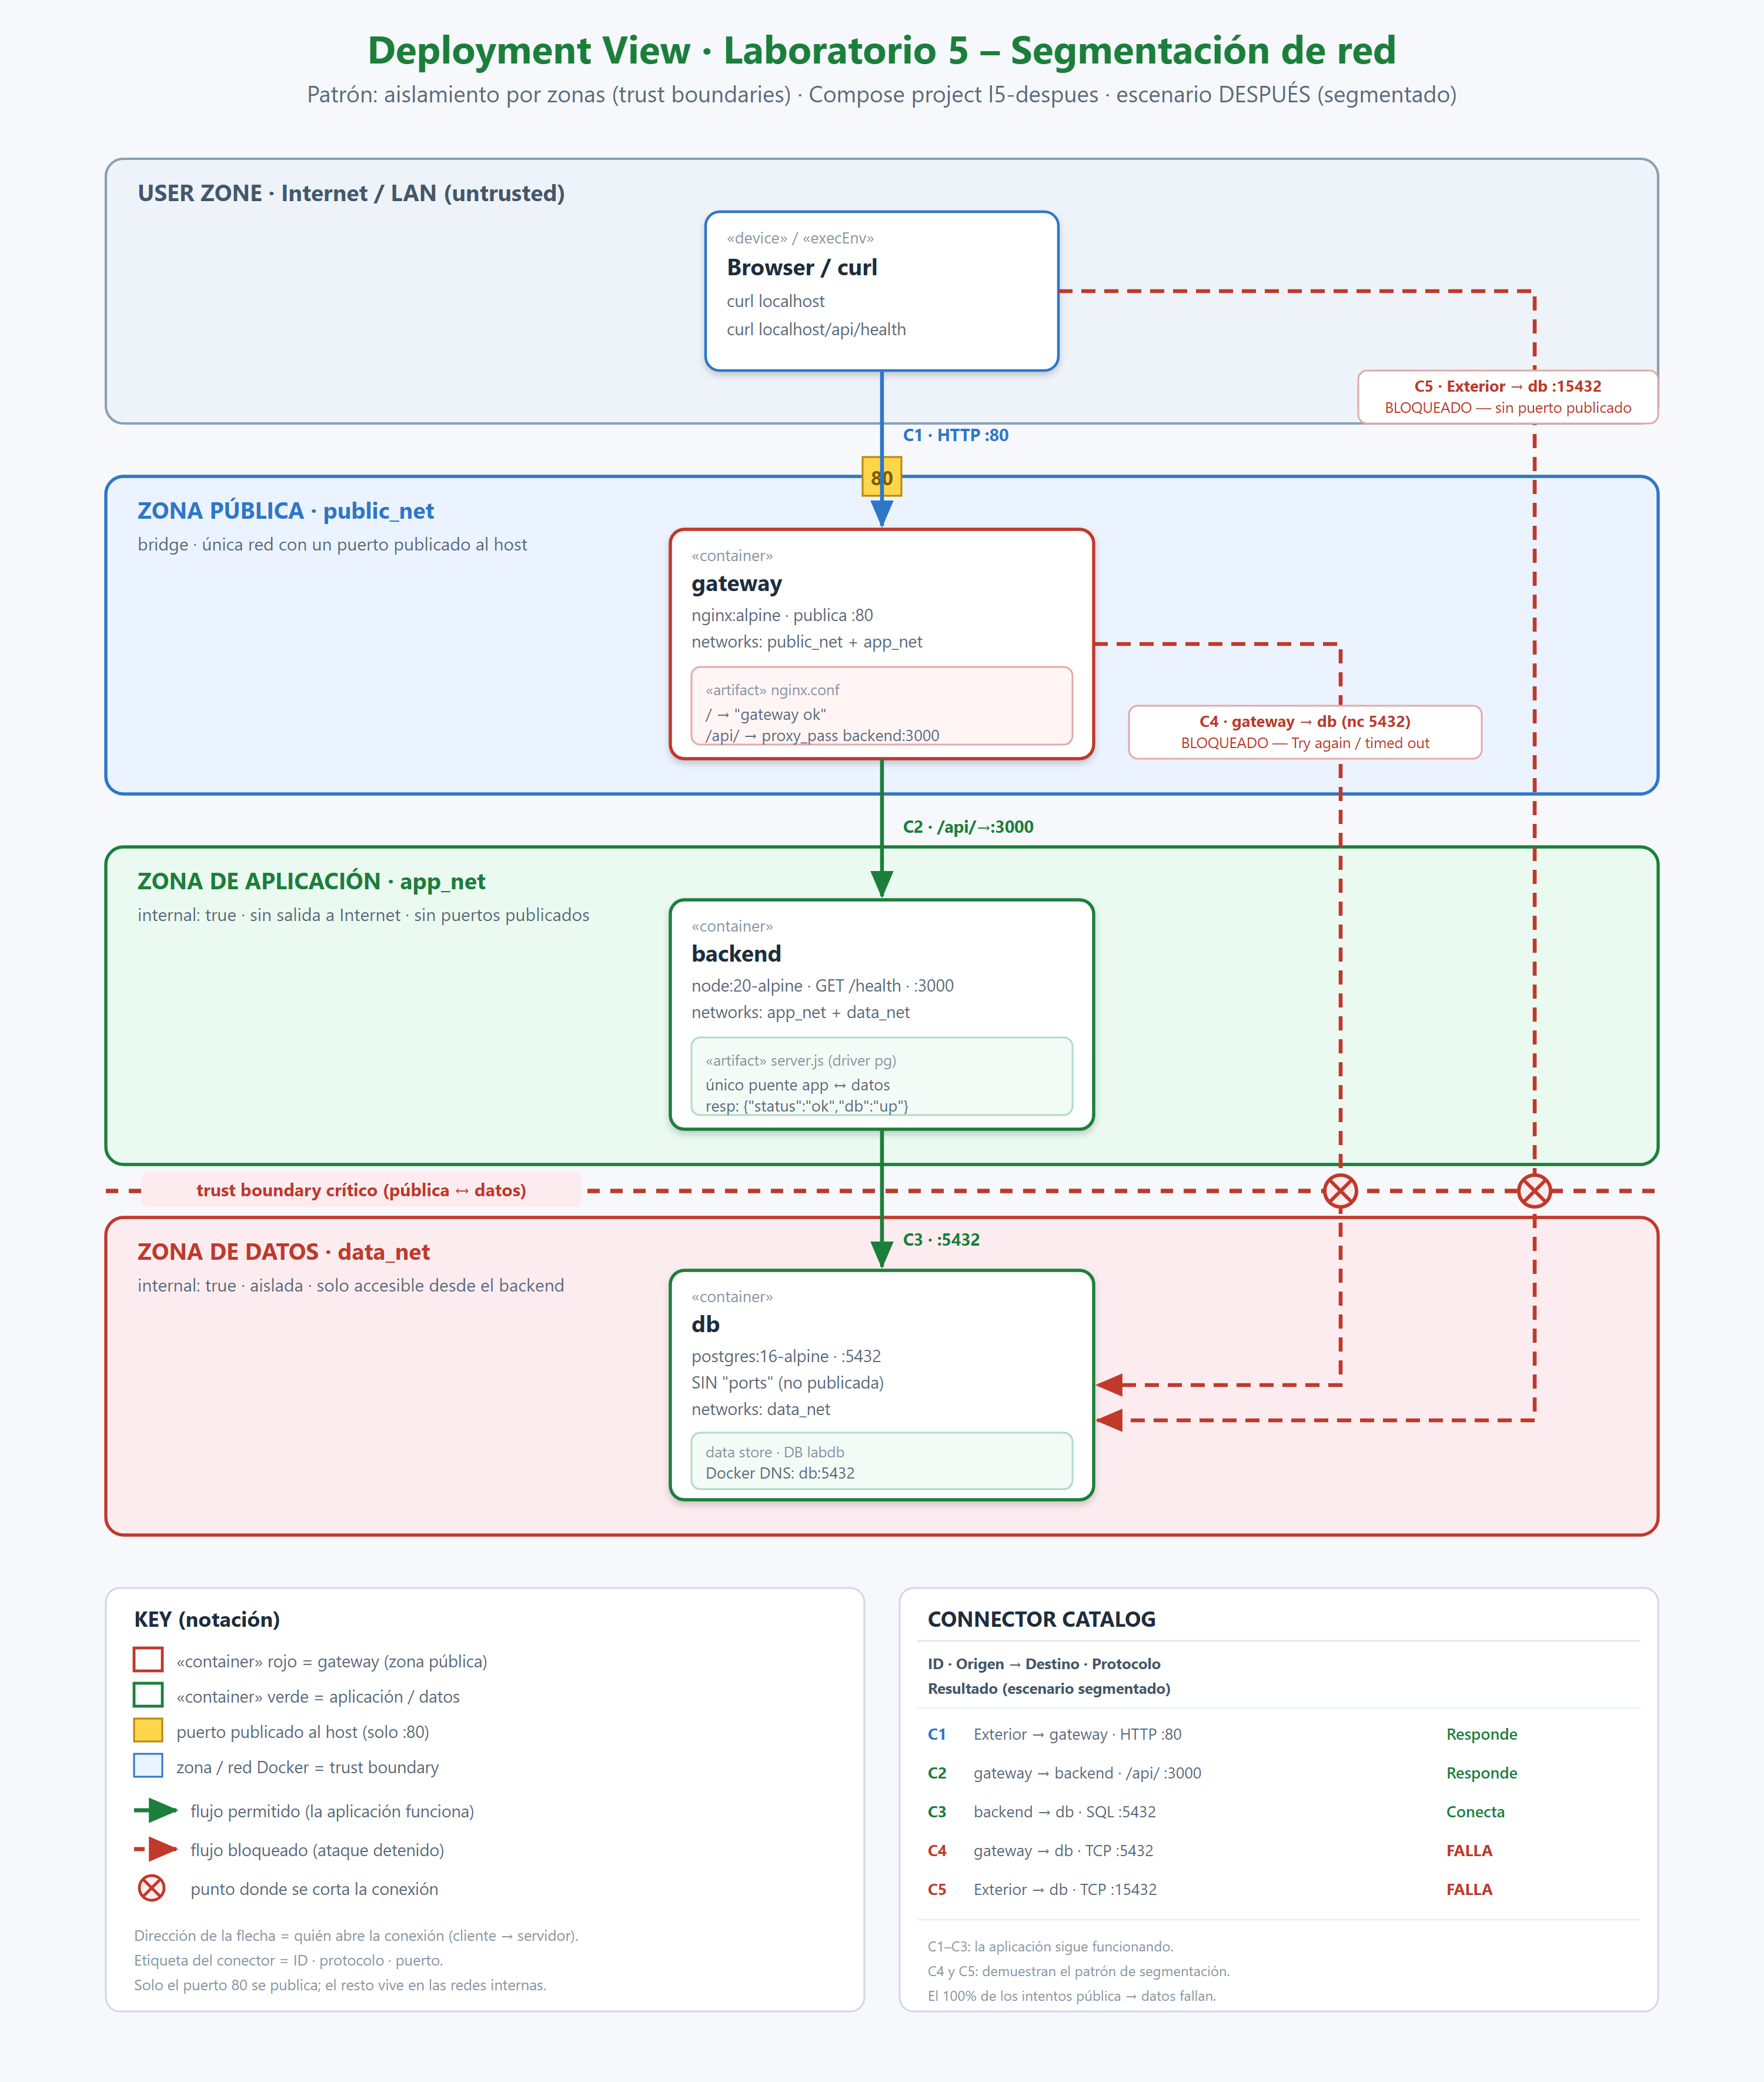
\includegraphics[width=0.92\textwidth,height=0.78\textheight,keepaspectratio]{vista-arquitectonica.png}
  \caption{Vista de despliegue con las zonas de confianza, los flujos permitidos y los flujos bloqueados.}
  \label{fig:vista}
\end{figure}

\begin{table}[H]
\centering
\small
\begin{tabularx}{\textwidth}{c l l Y}
\toprule
\rowcolor{headbg}
\textbf{ID} & \textbf{Origen → Destino} & \textbf{Resultado} & \textbf{Qué lo permite o lo bloquea} \\
\midrule
C1 & Exterior → gateway (HTTP :80)       & \ok{Responde} & Único puerto publicado (\code{ports: "80:80"}). \\
C2 & gateway → backend (HTTP :3000)      & \ok{Responde} & Ambos comparten \code{app\_net}. \\
C3 & backend → db (TCP :5432)            & \ok{Conecta}  & Ambos comparten \code{data\_net}. \\
C4 & gateway → db (TCP :5432)            & \bad{Falla}   & El gateway no tiene interfaz en \code{data\_net}: no resuelve \code{db} ni tiene ruta a su IP. \\
C5 & Exterior → db (TCP :15432)          & \bad{Falla}   & El servicio \code{db} no declara \code{ports}; el host no escucha en ese puerto. \\
\bottomrule
\end{tabularx}
\caption{Conectores de la vista y mecanismo que los habilita o los bloquea.}
\end{table}

% =====================================================================
\section{Implementación}

\subsection{Requisitos previos}

\begin{itemize}
  \item Docker Engine y Docker Compose v2 (se verificó con Docker 29.9.2 y Compose v5.6.1 sobre Windows 11).
  \item El puerto 80 libre en el host.
  \item PowerShell (Windows) o una terminal bash (Linux/macOS) para las pruebas.
\end{itemize}

El código completo está en el repositorio del equipo:
\url{https://github.com/svargasm21/L5_1F}.

\subsection{Estructura del proyecto}

\begin{lstlisting}
L5_1F/
+-- gateway/     nginx (zona pública): Dockerfile, nginx.conf
+-- backend/     Node.js + pg (zona de aplicación): Dockerfile, server.js
+-- antes/       docker-compose.yml -> una sola red, BD publicada al host
+-- despues/     docker-compose.yml -> tres redes segmentadas
+-- evidencia/   pruebas.ps1, antes.log, despues.log, RESULTADOS.md
\end{lstlisting}

Las mismas imágenes de \code{gateway} y \code{backend} se usan en los dos escenarios;
lo único que cambia entre el \emph{antes} y el \emph{después} es el archivo
\code{docker-compose.yml}.

\subsection{Paso 1: identificar zonas y flujos permitidos}

Antes de escribir configuración, el equipo definió las tres zonas de la
sección~1.3 y la lista de flujos legítimos: exterior → gateway, gateway → backend y
backend → db. Todo flujo que no esté en esa lista debe fallar. Esta lista es la que
después se convierte en redes de Docker.

\subsection{Paso 2: construir los componentes}

\textbf{Gateway (zona pública).} nginx responde en \code{/} y reenvía \code{/api/} al backend.

\textit{a.} \code{gateway/nginx.conf}
\begin{lstlisting}[language=nginx]
server {
    listen 80;

    # Prueba 1: el gateway responde al exterior
    location = / {
        default_type text/plain;
        return 200 "gateway ok\n";
    }

    # Flujo permitido: gateway -> backend
    location /api/ {
        proxy_pass http://backend:3000/;
    }
}
\end{lstlisting}

\textit{b.} \code{gateway/Dockerfile}
\begin{lstlisting}[language=docker]
FROM nginx:1.27-alpine
# curl y nc solo se instalan para ejecutar las pruebas del laboratorio
RUN apk add --no-cache curl netcat-openbsd
COPY nginx.conf /etc/nginx/conf.d/default.conf
\end{lstlisting}

\textbf{Backend (zona de aplicación).} API mínima con un endpoint \code{GET /health}
que consulta la base de datos, de modo que una respuesta \code{"db":"up"} demuestra
que la cadena completa funciona.

\textit{c.} \code{backend/server.js}
\begin{lstlisting}[language=JavaScript]
// API mínima: GET /health consulta la base de datos y responde su estado.
const http = require("http");
const { Pool } = require("pg");

const pool = new Pool({
  host: process.env.DB_HOST || "db",
  port: Number(process.env.DB_PORT || 5432),
  user: process.env.DB_USER,
  password: process.env.DB_PASSWORD,
  database: process.env.DB_NAME,
  connectionTimeoutMillis: 3000,
});

const send = (res, code, body) => {
  res.writeHead(code, { "Content-Type": "application/json" });
  res.end(JSON.stringify(body));
};

http
  .createServer(async (req, res) => {
    if (req.url !== "/health") return send(res, 404, { error: "not found" });
    try {
      const { rows } = await pool.query("SELECT NOW() AS now");
      send(res, 200, { status: "ok", db: "up", time: rows[0].now });
    } catch (err) {
      send(res, 503, { status: "error", db: "down", detail: err.message });
    }
  })
  .listen(3000, () => console.log("backend escuchando en :3000"));
\end{lstlisting}

\textit{d.} \code{backend/Dockerfile}
\begin{lstlisting}[language=docker]
FROM node:20-alpine
# curl y nc solo se instalan para ejecutar las pruebas del laboratorio
RUN apk add --no-cache curl netcat-openbsd
WORKDIR /app
COPY package.json .
RUN npm install --omit=dev
COPY server.js .
EXPOSE 3000
CMD ["node", "server.js"]
\end{lstlisting}

\textbf{Base de datos (zona de datos).} Se usa la imagen oficial \code{postgres:16-alpine}; no requiere código.

\subsection{Paso 3: montar la línea base sin segmentar}

Para tener contra qué comparar, primero se despliega el sistema como suele quedar
por defecto: todos los servicios en la red \code{default} del proyecto y la base de
datos publicada al host. Se usa el puerto 15432 en el host para no chocar con un
PostgreSQL local.

\code{antes/docker-compose.yml}
\begin{lstlisting}[language=yaml]
# ANTES: todos los servicios en la red por defecto y la BD publicada al host.
# Credenciales solo para el laboratorio.
name: l5-antes

services:
  gateway:
    build: ../gateway
    ports:
      - "80:80"
    depends_on:
      - backend

  backend:
    build: ../backend
    environment:
      DB_HOST: db
      DB_USER: lab
      DB_PASSWORD: lab_password
      DB_NAME: labdb
    depends_on:
      db:
        condition: service_healthy

  db:
    image: postgres:16-alpine
    environment:
      POSTGRES_USER: lab
      POSTGRES_PASSWORD: lab_password
      POSTGRES_DB: labdb
    ports:
      # Expuesta al exterior (mala práctica, a propósito).
      - "15432:5432"
    healthcheck:
      test: ["CMD-SHELL", "pg_isready -U lab -d labdb"]
      interval: 3s
      retries: 10
\end{lstlisting}

\subsection{Paso 4: declarar las redes segmentadas}

Este es el paso donde se aplica el patrón. Cada zona se convierte en una red de
Docker y cada servicio se conecta solo a las redes de su zona y de la zona contigua.

\code{despues/docker-compose.yml}
\begin{lstlisting}[language=yaml]
# DESPUÉS: patrón de segmentación de red en tres zonas.
#   public_net : zona pública  -> gateway
#   app_net    : zona de aplicación -> gateway, backend
#   data_net   : zona de datos -> backend, db
name: l5-despues

services:
  gateway:
    build: ../gateway
    ports:
      - "80:80"            # único puerto publicado al exterior
    networks:
      - public_net
      - app_net
    depends_on:
      - backend

  backend:
    build: ../backend
    environment:
      DB_HOST: db
      DB_USER: lab
      DB_PASSWORD: lab_password
      DB_NAME: labdb
    networks:
      - app_net
      - data_net
    depends_on:
      db:
        condition: service_healthy

  db:
    image: postgres:16-alpine
    environment:
      POSTGRES_USER: lab
      POSTGRES_PASSWORD: lab_password
      POSTGRES_DB: labdb
    # sin "ports": la BD no se publica al host
    networks:
      - data_net
    healthcheck:
      test: ["CMD-SHELL", "pg_isready -U lab -d labdb"]
      interval: 3s
      retries: 10

networks:
  public_net: {}
  app_net:
    internal: true         # sin salida a Internet
  data_net:
    internal: true         # sin salida a Internet
\end{lstlisting}

La segmentación se logra con tres decisiones:

\begin{enumerate}
  \item \textbf{Redes por zona.} \code{gateway} está en \code{public\_net} y \code{app\_net}; \code{backend} en \code{app\_net} y \code{data\_net}; \code{db} solo en \code{data\_net}. El gateway y la base de datos no comparten ninguna red.
  \item \textbf{Un solo puerto publicado.} Solo el gateway declara \code{ports}. Se eliminó \code{ports} del servicio \code{db}.
  \item \textbf{Redes internas.} \code{app\_net} y \code{data\_net} se marcan con \code{internal: true}, así que no tienen salida a Internet ni se pueden publicar al host.
\end{enumerate}

No hubo que cambiar el código de ningún servicio. El backend sigue usando
\code{DB\_HOST: db} porque el DNS interno de Docker resuelve el nombre dentro de
\code{data\_net}.

\subsection{Paso 5: desplegar y revisar las redes}

Ambos escenarios usan el puerto 80, así que se levantan uno a la vez.

\begin{lstlisting}[language=shell]
cd antes
docker compose up -d --build
# ... pruebas del paso 6 ...
docker compose down

cd ..\despues
docker compose up -d --build

# Redes creadas y redes de cada contenedor
docker network ls --filter name=l5-despues
docker inspect -f '{{range $k,$v := .NetworkSettings.Networks}}{{$k}} {{end}}' l5-despues-gateway-1
\end{lstlisting}

\subsection{Paso 6: ejecutar las pruebas}

Se ejecutan las mismas pruebas en ambos escenarios. Las pruebas 1 a 3 comprueban que
la aplicación sigue funcionando; las pruebas 4, 4b y 5 son las que demuestran el patrón.

\begin{lstlisting}[language=shell]
# 1. Exterior -> gateway (y cadena completa hasta la BD)
curl.exe localhost
curl.exe localhost/api/health
# 2. gateway -> backend
docker compose exec gateway curl -s backend:3000/health
# 3. backend -> db
docker compose exec backend nc -zv -w 3 db 5432
# 4. gateway -> db por nombre (debe fallar en el "después")
docker compose exec gateway nc -zv -w 3 db 5432
# 4b. gateway -> db por IP (descarta que el bloqueo sea solo de DNS)
$ip = docker inspect -f '{{range .NetworkSettings.Networks}}{{.IPAddress}}{{end}}' l5-despues-db-1
docker compose exec gateway nc -zv -w 3 $ip 5432
# 5. Exterior -> db  (en Linux/macOS: nc -zv localhost 15432)
Test-NetConnection localhost -Port 15432
\end{lstlisting}

Para repetir todo de forma automática, el script \code{evidencia/pruebas.ps1}
levanta cada escenario, ejecuta las pruebas, compara contra el resultado esperado,
guarda la salida en \code{antes.log} y \code{despues.log} y apaga los contenedores:

\begin{lstlisting}[language=shell]
powershell -ExecutionPolicy Bypass -File evidencia\pruebas.ps1
# Opciones: -Escenario despues   (solo un escenario)
#           -NoApagar            (deja los contenedores arriba para capturas)
\end{lstlisting}

% =====================================================================
\section{Resultados}

\subsection{Comparación antes y después}

Ejecución del 9 de noviembre de 2026. En verde, el resultado deseado; en rojo, un
flujo que no debería existir y conecta.

\begin{table}[H]
\centering
\small
\begin{tabularx}{\textwidth}{c l Y Y}
\toprule
\rowcolor{headbg}
\textbf{\#} & \textbf{Desde → hacia} & \textbf{Antes (una red)} & \textbf{Después (segmentado)} \\
\midrule
1  & Exterior → gateway           & \ok{Responde} \code{gateway ok}            & \ok{Responde} \code{gateway ok} \\
1b & Exterior → gateway → backend → db & \ok{Responde} \code{"db":"up"}       & \ok{Responde} \code{"db":"up"} \\
2  & gateway → backend            & \ok{Responde} \code{"db":"up"}             & \ok{Responde} \code{"db":"up"} \\
3  & backend → db                 & \ok{Conecta} \code{succeeded!}             & \ok{Conecta} \code{succeeded!} \\
4  & gateway → db (nombre)        & \bad{Conecta} \code{succeeded!}            & \ok{Falla} \code{getaddrinfo: Try again} \\
4b & gateway → db (IP)            & \bad{Conecta} \code{succeeded!}            & \ok{Falla} \code{timed out} \\
5  & Exterior → db (:15432)       & \bad{Conecta} \code{True}                  & \ok{Falla} \code{False} \\
\bottomrule
\end{tabularx}
\caption{Resultados de las pruebas en ambos escenarios.}
\end{table}

\subsection{Evidencia clave: la misma prueba desde dos zonas}

En el escenario segmentado, el gateway no llega a la base de datos ni por nombre ni
por IP, mientras que el backend sí:

\begin{lstlisting}[language=shell]
PS> docker compose exec gateway nc -zv -w 3 db 5432
nc: getaddrinfo for host "db" port 5432: Try again

PS> docker compose exec gateway nc -zv -w 3 172.23.0.2 5432
nc: connect to 172.23.0.2 port 5432 (tcp) timed out: Operation in progress

PS> docker compose exec backend nc -zv -w 3 db 5432
Connection to db (172.23.0.2) 5432 port [tcp/postgresql] succeeded!
\end{lstlisting}

Redes de cada contenedor y puertos publicados al host:

\begin{table}[H]
\centering
\small
\begin{tabularx}{\textwidth}{l Y l l}
\toprule
\rowcolor{headbg}
\textbf{Servicio} & \textbf{Redes (después)} & \textbf{Puerto en el host (antes)} & \textbf{Puerto en el host (después)} \\
\midrule
gateway & \code{public\_net}, \code{app\_net} & 80 & 80 \\
backend & \code{app\_net}, \code{data\_net}   & ninguno & ninguno \\
db      & \code{data\_net}                    & \bad{15432} & \ok{ninguno} \\
\bottomrule
\end{tabularx}
\caption{Redes y puertos publicados por servicio.}
\end{table}

\subsection{Mejoras observadas}

\begin{itemize}
  \item \textbf{Medida del escenario cumplida.} En el \emph{después} fallan los 3 intentos de llegar a la base de datos sin pasar por el backend (pruebas 4, 4b y 5): \textbf{3/3 = 100\,\%}. En el \emph{antes} los 3 conectaban (0\,\% bloqueado).
  \item \textbf{La aplicación sigue funcionando.} Las pruebas 1, 1b, 2 y 3 dan el mismo resultado en los dos escenarios.
  \item \textbf{El bloqueo no depende solo del DNS.} La prueba 4 falla porque el gateway no resuelve \code{db}. La 4b muestra que, aun conociendo la IP, el paquete no tiene ruta porque el gateway no tiene interfaz en \code{data\_net}.
  \item \textbf{Menor superficie de ataque externa.} Los puertos publicados al host pasan de dos (80 y 15432) a uno (80).
  \item \textbf{Menos caminos hacia los datos.} En el \emph{antes}, tres orígenes llegaban a la base de datos (exterior, gateway y backend); en el \emph{después}, solo el backend.
  \item \textbf{Costo de adopción bajo.} El cambio se hizo solo en \code{docker-compose.yml}; no se modificó código de la aplicación.
\end{itemize}

% =====================================================================
\section{Recomendaciones para replicar el patrón}

\subsection{Diseño}

\begin{itemize}
  \item \textbf{Empezar por la lista de flujos permitidos}, no por el YAML. Si un flujo no está en la lista, no debe existir una red compartida que lo habilite.
  \item \textbf{Una red por zona, no por servicio.} Los servicios puente se conectan como máximo a dos redes: la de su zona y la contigua.
  \item \textbf{Publicar solo el punto de entrada.} Quitar \code{ports} de bases de datos y servicios internos. Para depurar, usar un archivo aparte que se carga a mano (\code{docker compose -f docker-compose.yml -f debug.yml up}) en lugar de dejar puertos abiertos en el archivo principal.
  \item \textbf{Marcar las redes internas con \code{internal: true}.} Hay que tener en cuenta que esto corta la salida a Internet: si un servicio necesita una API externa, se le agrega una red de salida propia en vez de quitar \code{internal}. La construcción de imágenes (\code{build}) no se ve afectada.
\end{itemize}

\subsection{Pruebas}

\begin{itemize}
  \item \textbf{Probar el bloqueo por IP, además de por nombre.} Que un nombre no se resuelva no prueba que no haya ruta.
  \item \textbf{Usar siempre un tiempo límite} (\code{nc -w 3}). Sin él, la prueba por IP se queda colgada unos dos minutos.
  \item \textbf{Evitar falsos positivos en la prueba 5.} Si el \emph{después} da \code{True}, hay otro proceso escuchando en ese puerto del host (por ejemplo, un PostgreSQL local). Por eso el \emph{antes} publica la BD en el 15432. Se revisa con \code{Get-NetTCPConnection -LocalPort 15432}.
  \item \textbf{PowerShell 5.1 y \code{nc}.} \code{nc -zv} escribe en \emph{stderr}; conviene redirigir dentro del contenedor (\code{sh -c "nc -zv ... 2>\&1"}) para que la salida no aparezca como error.
  \item \textbf{No dejar herramientas de red en producción.} \code{curl} y \code{nc} se instalaron solo para el laboratorio. En producción es mejor probar con un contenedor temporal conectado a la red (por ejemplo, \code{docker run -{}-rm -{}-network <red> nicolaka/netshoot}).
\end{itemize}

\subsection{Alcance del patrón}

\begin{itemize}
  \item \textbf{La segmentación no reemplaza la autenticación.} El backend sí llega a la BD, así que si se compromete el backend los datos quedan expuestos. Las credenciales deben salir del YAML (secretos de Docker o variables fuera del repositorio) y el patrón se complementa con \emph{Reverse Proxy} (el gateway ya cumple ese rol) y \emph{Secure Channel} (TLS entre zonas).
  \item \textbf{El mismo diseño aplica en otras plataformas.} En Kubernetes se implementa con \code{NetworkPolicy} (denegar todo por defecto y permitir solo los flujos de la lista); en la nube, con subredes y grupos de seguridad.
\end{itemize}

\subsection{Aplicación al proyecto BOLOLó}

Según la entrega del prototipo 2, BOLOLó ya separa una red pública
(\code{bololo-integrado\_public}), donde solo el gateway publica el puerto 80, de una
red privada (\code{bololo-integrado\_internal}) donde conviven todos los servicios y
las bases de datos. El siguiente paso que proponemos es dividir esa red privada como
en este laboratorio:

\begin{itemize}
  \item Una red de aplicación con \code{bololo\_lobby}, \code{bololo\_game}, \code{bololo\_auth}, \code{bololo\_ratings}, \code{bololo\_bots} y el broker \code{bololo\_mq}.
  \item Una red de datos por servicio (por ejemplo, \code{auth\_data} con \code{bololo\_auth} y \code{bololo\_auth\_db}). Así cada microservicio solo alcanza su propia base de datos, y la regla de \emph{una base de datos por servicio} queda impuesta por la red y no solo por convención.
\end{itemize}

% =====================================================================
\section{Conclusiones}

El patrón de segmentación de red se implementó en Docker Compose con tres redes, un
solo puerto publicado y sin cambios en el código. Las pruebas muestran que el
escenario de confidencialidad se cumple: el 100\,\% de los intentos de llegar a la
base de datos desde la zona pública o el exterior fallan, mientras que todos los
flujos legítimos siguen funcionando. Como el cambio está en la configuración de
despliegue, otros equipos pueden replicarlo en sus proyectos siguiendo los pasos de
la sección~4.

% =====================================================================
\section*{Referencias}
\addcontentsline{toc}{section}{Referencias}

\begin{itemize}[leftmargin=*]
  \item Bass, L., Clements, P. y Kazman, R. (2021). \emph{Software Architecture in Practice} (4.\textsuperscript{a} ed.). Addison-Wesley.
  \item Docker Inc. \emph{Networks top-level elements} (referencia de Compose). \url{https://docs.docker.com/reference/compose-file/networks/}
  \item Docker Inc. \emph{Networking in Compose}. \url{https://docs.docker.com/compose/how-tos/networking/}
  \item The Kubernetes Authors. \emph{Network Policies}. \url{https://kubernetes.io/docs/concepts/services-networking/network-policies/}
\end{itemize}

\end{document}
